\documentclass[11pt,a4paper]{article}
\usepackage[utf8]{inputenc}
\usepackage[T1]{fontenc}
\usepackage[brazilian,provide=*]{babel}
\usepackage[margin=2.5cm]{geometry}
\usepackage{amsmath}
\usepackage{xcolor}
\usepackage{graphicx}
\usepackage{booktabs}
\usepackage{array}
\usepackage{listings}
\usepackage{float}
\usepackage{adjustbox}
\usepackage{tikz}
\usetikzlibrary{positioning,arrows.meta,calc}
\graphicspath{{generated/}}

\setlength{\parindent}{0pt}
\setlength{\parskip}{0.55em}
\newcolumntype{L}[1]{>{\raggedright\arraybackslash}p{#1}}
\lstset{basicstyle=\ttfamily\footnotesize, breaklines=true, frame=single, columns=fullflexible, keepspaces=true}

\title{\textbf{Mini-Pilha de Rede em Camadas}\\[0.3em]
\large Trabalho Pr\'atico 2: implementa\c{c}\~ao em C sobre soquetes UDP}
\author{Kevin Miyahara Omori \\ Programa de Gradua\c{c}\~ao em Ci\^encia da Computa\c{c}\~ao, IME-USP}
\date{Outubro de 2026}

\begin{document}
\maketitle

\section{Arquitetura do sistema}

A mini-pilha \'e um programa em C (\texttt{ministack}) que implementa quatro camadas independentes: aplica\c{c}\~ao, transporte, rede e enlace. Cada inst\^ancia do programa \'e um n\'o da rede, identificado por um endere\c{c}o l\'ogico de 16 bits. Os n\'os conversam por soquetes UDP reais, mas o enlace \'e simulado: o soquete UDP faz o papel do meio f\'isico, e a camada de enlace decide, para cada frame, se ele \'e perdido, atrasado ou corrompido antes de chegar ao vizinho.

\begin{figure}[H]
\centering
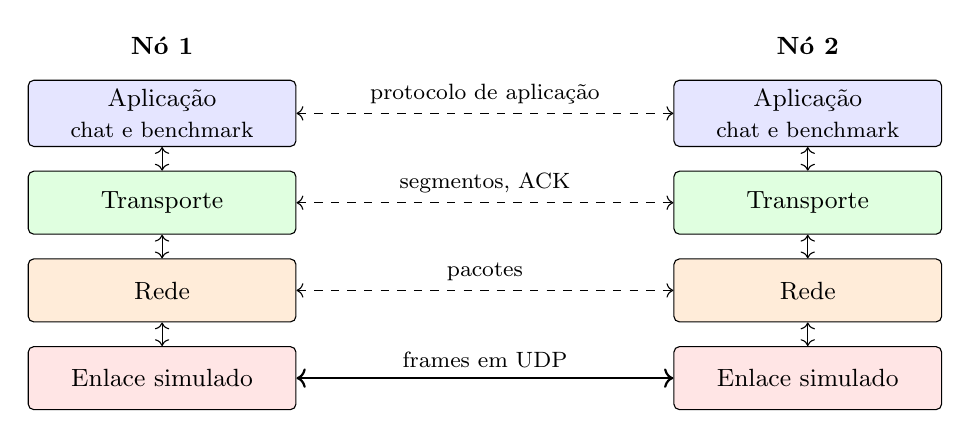
\begin{tikzpicture}[font=\small,
  layer/.style={draw, rounded corners=2pt, minimum width=3.4cm, minimum height=0.8cm, align=center},
  app/.style={layer, fill=blue!10}, trp/.style={layer, fill=green!12},
  net/.style={layer, fill=orange!15}, lnk/.style={layer, fill=red!10}]
\node[app] (a4) at (0,0) {Aplica\c{c}\~ao\\{\footnotesize chat e benchmark}};
\node[trp, below=3mm of a4] (a3) {Transporte};
\node[net, below=3mm of a3] (a2) {Rede};
\node[lnk, below=3mm of a2] (a1) {Enlace simulado};
\node[app] (b4) at (8.2,0) {Aplica\c{c}\~ao\\{\footnotesize chat e benchmark}};
\node[trp, below=3mm of b4] (b3) {Transporte};
\node[net, below=3mm of b3] (b2) {Rede};
\node[lnk, below=3mm of b2] (b1) {Enlace simulado};
\node[above=2mm of a4] {\textbf{N\'o 1}};
\node[above=2mm of b4] {\textbf{N\'o 2}};
\path (a4) edge[<->, dashed] node[above] {\footnotesize protocolo de aplica\c{c}\~ao} (b4);
\path (a3) edge[<->, dashed] node[above] {\footnotesize segmentos, ACK} (b3);
\path (a2) edge[<->, dashed] node[above] {\footnotesize pacotes} (b2);
\path (a1) edge[<->, thick] node[above] {\footnotesize frames em UDP} (b1);
\foreach \x in {a,b} {
  \path (\x4) edge[<->] (\x3);
  \path (\x3) edge[<->] (\x2);
  \path (\x2) edge[<->] (\x1);
}
\end{tikzpicture}
\caption{Pilha de dois n\'os. Cada camada conversa apenas com a vizinha no mesmo n\'o (setas cheias) e, logicamente, com a camada par do outro n\'o (setas tracejadas).}
\end{figure}

Cada n\'o \'e um \'unico processo com um la\c{c}o de eventos baseado em \texttt{select}: ele espera o soquete UDP, a entrada padr\~ao (no modo chat) e o pr\'oximo prazo de qualquer camada (temporizador de retransmiss\~ao do transporte, frames retidos pelo atraso simulado, pr\'oxima mensagem agendada da aplica\c{c}\~ao). Com isso n\~ao h\'a \emph{threads} nem travas, e o comportamento de cada camada \'e determin\'istico dado o mesmo conjunto de eventos.

A mesma pilha suporta mais de dois n\'os: o endere\c{c}amento da camada de rede e a tabela de rotas est\'atica permitem que um n\'o intermedi\'ario encaminhe pacotes entre dois outros, como nos testes de tr\^es n\'os da Se\c{c}\~ao~7.

\textbf{Siglas.} UDP (\emph{User Datagram Protocol}); TTL (\emph{time to live}, n\'umero m\'aximo de saltos de um pacote); CRC (\emph{cyclic redundancy check}, c\'odigo de detec\c{c}\~ao de erros); ACK (\emph{acknowledgement}, confirma\c{c}\~ao de recebimento); RTT (\emph{round-trip time}, tempo de ida e volta); RTO (\emph{retransmission timeout}, temporizador de retransmiss\~ao); KiB (\emph{kibibyte}, 1024 bytes).

\begin{table}[H]
\centering\small
\begin{tabular}{lll}
\toprule
\textbf{Arquivo} & \textbf{Camada} & \textbf{Conte\'udo} \\
\midrule
\texttt{src/application.c} & Aplica\c{c}\~ao & chat com sess\~ao; aplica\c{c}\~ao de benchmark \\
\texttt{src/transport.c} & Transporte & portas, numera\c{c}\~ao, ACK, retransmiss\~ao, modo n\~ao confi\'avel \\
\texttt{src/network.c} & Rede & endere\c{c}os, cabe\c{c}alho, rotas est\'aticas, TTL, encaminhamento \\
\texttt{src/link.c} & Enlace & frame, CRC-16, perda, atraso, jitter, corrup\c{c}\~ao; soquete UDP \\
\texttt{src/node.c} & Integra\c{c}\~ao & op\c{c}\~oes, liga\c{c}\~ao entre camadas, la\c{c}o de eventos \\
\texttt{src/common.c} & Apoio & rel\'ogio, leitura e escrita de inteiros em ordem de rede, trace \\
\bottomrule
\end{tabular}
\caption{Organiza\c{c}\~ao do c\'odigo-fonte. Os cabe\c{c}alhos p\'ublicos ficam em \texttt{include/}.}
\end{table}

\section{Responsabilidades de cada camada}

\subsection{Aplica\c{c}\~ao}

Duas aplica\c{c}\~oes compartilham o mesmo n\'o, cada uma em sua porta l\'ogica. O \textbf{chat} (porta 1) tem protocolo pr\'oprio com controle de sess\~ao: um n\'o abre a sess\~ao com \texttt{HELLO}, o outro confirma com \texttt{HELLO\_ACK}, e s\'o depois mensagens \texttt{TEXT} s\~ao aceitas; \texttt{BYE} encerra a sess\~ao. Texto recebido fora de uma sess\~ao estabelecida \'e rejeitado e contado. O \textbf{benchmark} (porta 2) envia uma quantidade configur\'avel de mensagens numeradas, com conte\'udo determin\'istico, e o receptor confere ordem, duplicatas, lacunas e integridade do conte\'udo; \'e ele que torna os experimentos mensur\'aveis.

\subsection{Transporte}

Respons\'avel pela comunica\c{c}\~ao entre processos. Identifica origem e destino por portas l\'ogicas, o que multiplexa v\'arias aplica\c{c}\~oes sobre o mesmo endere\c{c}o de rede. No modo confi\'avel, numera os segmentos, mant\'em uma janela deslizante, confirma o recebimento com ACK cumulativo e retransmite quando o temporizador expira. No modo n\~ao confi\'avel, envia os segmentos numerados sem ACK, e o receptor apenas contabiliza lacunas. Se uma mensagem esgota o limite de retransmiss\~oes, o transporte avisa a aplica\c{c}\~ao.

\subsection{Rede}

Identifica n\'os e entrega pacotes. Cada pacote carrega endere\c{c}o de origem, de destino e um TTL. Se o destino \'e o pr\'oprio n\'o, o segmento sobe ao transporte; caso contr\'ario, o pacote \'e encaminhado pelo vizinho indicado na tabela de rotas, com o TTL decrementado, e \'e descartado quando o TTL se esgota ou n\~ao h\'a rota.

\subsection{Enlace (simulado)}

Constr\'oi o frame (tamanho e CRC-16 de 16 bits), entrega-o ao vizinho por UDP e simula as imperfei\c{c}\~oes do meio: perda, atraso fixo, jitter e corrup\c{c}\~ao de bits, todos configur\'aveis por op\c{c}\~ao de linha de comando e com semente \emph{pseudoaleat\'oria} fixa para reprodutibilidade. No recebimento, valida o tamanho e o CRC e descarta frames inv\'alidos. A verifica\c{c}\~ao do CRC pode ser desligada, o que permite medir o valor da detec\c{c}\~ao de erros.

\section{Interfaces entre camadas}

A regra de separa\c{c}\~ao \'e estrutural: cada camada s\'o inclui o cabe\c{c}alho da camada imediatamente abaixo e chama apenas as primitivas dela. A comunica\c{c}\~ao para cima usa \emph{callbacks}: o m\'odulo de integra\c{c}\~ao (\texttt{node.c}), o \'unico que conhece todas as camadas, liga o enlace \`a rede e a rede ao transporte, e a pr\'opria aplica\c{c}\~ao registra os seus no transporte com \texttt{tp\_bind}. Assim, nenhuma camada depende da implementa\c{c}\~ao da que est\'a acima. Um teste autom\'atico confere as inclus\~oes de cada m\'odulo (Se\c{c}\~ao~7.7).

\begin{table}[H]
\centering\small
\begin{tabular}{L{2.6cm}L{6.2cm}L{5.0cm}}
\toprule
\textbf{Interface} & \textbf{Primitivas (para baixo)} & \textbf{\emph{Callback} (para cima)} \\
\midrule
Aplica\c{c}\~ao e transporte & \texttt{tp\_bind(porta, on\_data, on\_error)}, \texttt{tp\_send(porta, destino, porta\_destino, dados, tamanho, confi\'avel)}, \texttt{tp\_pending()} & \texttt{tp\_data\_fn(origem, porta, dados, tamanho)}, \texttt{tp\_error\_fn(destino, porta, erro)} \\
Transporte e rede & \texttt{net\_send(destino, segmento, tamanho)} & \texttt{net\_rx\_fn(origem, segmento, tamanho)}, registrado com \texttt{net\_set\_upper} \\
Rede e enlace & \texttt{link\_send(vizinho, pacote, tamanho)} & \texttt{link\_rx\_fn(vizinho, pacote, tamanho)}, registrado com \texttt{link\_set\_upper} \\
Enlace e meio & \texttt{sendto} e \texttt{recvfrom} sobre UDP & \texttt{link\_on\_readable()} chamado pelo la\c{c}o de eventos \\
\bottomrule
\end{tabular}
\caption{Interfaces entre camadas. Os contratos completos est\~ao nos cabe\c{c}alhos de \texttt{include/}.}
\end{table}

Al\'em das primitivas de dados, cada camada com estado temporal exp\~oe \texttt{*\_tick(agora)} e \texttt{*\_next\_deadline()}, que o la\c{c}o de eventos usa para acordar no momento certo. O retorno de \texttt{tp\_send} distingue fila cheia, argumento inv\'alido e fluxo j\'a encerrado por falha, de modo que a aplica\c{c}\~ao reage a cada caso.

\section{Formato dos cabe\c{c}alhos e encapsulamento}

Todos os campos multi-byte usam ordem de rede (\emph{big-endian}) e s\~ao escritos e lidos byte a byte, sem convers\~ao direta de estruturas, o que evita depend\^encia de alinhamento ou de ordem de bytes da m\'aquina.

\begin{table}[H]
\centering\small
\begin{tabular}{lcL{9.2cm}}
\toprule
\textbf{Camada} & \textbf{Bytes} & \textbf{Campos (em bytes)} \\
\midrule
Enlace & 4 & tamanho do pacote (2); CRC-16 (2), calculado sobre o cabe\c{c}alho, com o campo do CRC zerado, e o pacote; polin\^omio 0x1021, valor inicial 0xFFFF \\
Rede & 9 & vers\~ao (1); TTL (1); origem (2); destino (2); protocolo (1); tamanho do segmento (2) \\
Transporte & 13 & porta de origem (2); porta de destino (2); n\'umero de sequ\^encia (4); n\'umero de confirma\c{c}\~ao (4); flags (1): \texttt{DATA} 0x01, \texttt{ACK} 0x02, \texttt{REL} 0x04 \\
Chat & 1 + texto & tipo (1): \texttt{HELLO} 1, \texttt{HELLO\_ACK} 2, \texttt{TEXT} 3, \texttt{BYE} 4; texto de at\'e 200 bytes \\
Benchmark & 5 + padr\~ao & tipo (1) igual a 10; identificador da mensagem (4); bytes de padr\~ao: XOR dos 4 bytes do identificador, mais o \'indice do byte, m\'odulo 256 \\
\bottomrule
\end{tabular}
\caption{Formato dos cabe\c{c}alhos de cada camada e das mensagens das aplica\c{c}\~oes.}
\end{table}

O n\'umero de confirma\c{c}\~ao de um ACK indica o pr\'oximo n\'umero de sequ\^encia esperado (ACK cumulativo). A flag \texttt{REL} marca os segmentos do modo confi\'avel, que s\~ao confirmados e ordenados; sem ela o segmento segue o caminho n\~ao confi\'avel.

O encapsulamento \'e progressivo: cada camada recebe os dados da superior como carga \'util opaca e acrescenta o pr\'oprio cabe\c{c}alho; no receptor, cada camada valida e remove o seu cabe\c{c}alho e entrega o restante \`a de cima. A Figura~\ref{fig:encap} mostra o resultado para a mensagem de chat ``ola bob'' e o trecho abaixo reproduz o trace real emitido com a op\c{c}\~ao \texttt{-v} (comando \texttt{python3 scripts/demo\_chat.py}), com os tempos omitidos. As mensagens do programa s\~ao ASCII, sem acentos, para n\~ao depender da codifica\c{c}\~ao do terminal.

\begin{figure}[H]
\centering
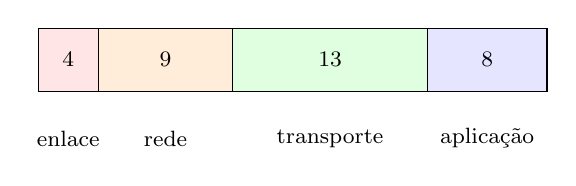
\begin{tikzpicture}[font=\small, x=0.19cm,
  box/.style={draw, minimum height=0.8cm, inner sep=0pt, align=center}]
\node[box, fill=red!10, minimum width=4*0.19cm] at (2,0) {};
\node[box, fill=orange!15, minimum width=9*0.19cm] at (8.5,0) {};
\node[box, fill=green!12, minimum width=13*0.19cm] at (19.5,0) {};
\node[box, fill=blue!10, minimum width=8*0.19cm] at (30,0) {};
\node at (2,-1) {\footnotesize enlace};
\node at (8.5,-1) {\footnotesize rede};
\node at (19.5,-1) {\footnotesize transporte};
\node at (30,-1) {\footnotesize aplica\c{c}\~ao};
\node at (2,0) {\footnotesize 4};
\node at (8.5,0) {\footnotesize 9};
\node at (19.5,0) {\footnotesize 13};
\node at (30,0) {\footnotesize 8};
\end{tikzpicture}
\caption{Frame de 34 bytes que transporta a mensagem de chat de 8 bytes (1 de tipo e 7 de texto): 4 + 9 + 13 + 8.}
\label{fig:encap}
\end{figure}

\begin{lstlisting}
APP SEND chat TEXT "ola bob"  (1 B de tipo + 7 B de texto) -> no 2 porta 1
TRP SEND sport=1 dport=1 seq=1 ack=0 flags=DATA|REL  cabecalho 13 B + carga 8 B
NET SEND src=1 dst=2 ttl=16 proto=1 len=21  cabecalho 9 B + segmento 21 B, proximo salto 2
LNK SEND len=30 crc=0xa597  cabecalho 4 B + carga 30 B = frame 34 B -> vizinho 2
  ... no receptor, o caminho inverso (o exemplo abaixo e o recebimento de um HELLO_ACK):
LNK RECV frame 30 B, CRC ok -> pacote de 26 B para a camada de rede
NET RECV src=2 dst=1 ttl=16 proto=1 -> segmento de 17 B para o transporte
TRP RECV sport=1 dport=1 seq=0 ack=0 flags=DATA|REL  carga 4 B
APP RECV chat HELLO_ACK "bob" de 2
\end{lstlisting}

\section{Decis\~oes de projeto}

\textbf{Soquetes UDP como meio f\'isico.} UDP preserva a fronteira dos datagramas e n\~ao acrescenta confiabilidade, o que deixa toda a confiabilidade a cargo do transporte implementado. Cada frame \'e exatamente um datagrama.

\textbf{Janela deslizante com ACK cumulativo (\emph{go-back-N}).} \'E a forma mais simples de manter v\'arios segmentos em voo e ainda assim ter retransmiss\~ao correta: o receptor s\'o aceita o segmento esperado e o emissor mant\'em um \'unico temporizador, para o segmento mais antigo sem confirma\c{c}\~ao. Em contrapartida, uma perda faz a janela inteira ser reenviada, custo medido na Se\c{c}\~ao~7.1. A janela 1 equivale a \emph{stop-and-wait}.

\textbf{Temporizador fixo.} O tempo de retransmiss\~ao \'e configur\'avel e constante, sem \emph{backoff} nem estimativa adaptativa do RTT. Isso mant\'em os experimentos interpret\'aveis; o RTT \'e apenas medido (amostras s\'o de segmentos n\~ao retransmitidos).

\textbf{Falha expl\'icita.} Ap\'os um n\'umero configur\'avel de retransmiss\~oes do mesmo segmento, o fluxo \'e encerrado e a aplica\c{c}\~ao \'e avisada, em vez de tentar para sempre.

\textbf{CRC-16 no enlace.} A detec\c{c}\~ao de erros fica no enlace, como em redes reais, e \'e verificada a cada salto. Frames inv\'alidos s\~ao descartados e tratados pelo transporte como perda.

\textbf{Aplica\c{c}\~ao de benchmark com conte\'udo verific\'avel.} O padr\~ao de bytes depende do identificador da mensagem, ent\~ao o receptor consegue distinguir uma mensagem perdida de uma corrompida que atravessou as camadas.

\textbf{Roteamento est\'atico com TTL.} Dispensa algoritmos de roteamento, mas mant\'em o encaminhamento entre n\'os e protege contra la\c{c}os.

\textbf{Reprodutibilidade.} Perda, atraso, jitter e corrup\c{c}\~ao usam gerador pseudoaleat\'orio com semente informada na linha de comando; os experimentos e as figuras s\~ao gerados por scripts a partir de arquivos CSV.

\section{Metodologia experimental}

Os experimentos rodam dois n\'os (emissor e receptor) em processos separados na mesma m\'aquina, comunicando-se pela interface de \emph{loopback}, em Linux com um \'unico n\'ucleo de CPU. O emissor executa o benchmark, que envia $N$ mensagens e termina quando todas foram confirmadas (modo confi\'avel) ou enviadas (modo n\~ao confi\'avel). A perda, o atraso e a corrup\c{c}\~ao s\~ao aplicados por cada n\'o aos frames que ele envia, portanto afetam tanto os dados quanto os ACKs.

\textbf{M\'etricas.} \emph{Tempo de conclus\~ao}: do envio da primeira mensagem \`a confirma\c{c}\~ao da \'ultima. \emph{Taxa de retransmiss\~ao}: retransmiss\~oes divididas pelo total de segmentos de dados transmitidos, incluindo as retransmiss\~oes. \emph{Mensagens entregues}: mensagens distintas e \'integras vistas pela aplica\c{c}\~ao receptora. \emph{Overhead}: bytes enviados ao enlace (nos dois sentidos) divididos pelos bytes entregues pela aplica\c{c}\~ao ao transporte. O RTT \'e medido pelo transporte entre o envio e o ACK de segmentos n\~ao retransmitidos.

\textbf{Par\^ametros-base.} $N = 100$ mensagens de 100 bytes, janela 4, temporizador de 60~ms, atraso de 5~ms por frame, tr\^es sementes (1, 2 e 3). Cada experimento varia um fator e mant\'em os demais fixos; os resultados s\~ao m\'edia e desvio padr\~ao amostral das tr\^es repeti\c{c}\~oes. Repetir uma execu\c{c}\~ao com a mesma semente reproduz a sequ\^encia de perdas, mas n\~ao a ordem exata dos eventos no tempo. Refazendo todos os experimentos do zero (140 execu\c{c}\~oes em 66 configura\c{c}\~oes), as contagens (retransmiss\~oes, mensagens entregues, bytes no enlace, frames rejeitados pelo CRC e mensagens adulteradas) coincidiram exatamente com as dos arquivos de \texttt{results/}, e os tempos m\'edios diferiram cerca de 1\% ou menos nos experimentos de perda, de corrup\c{c}\~ao, de janela e perda e no modo confi\'avel da compara\c{c}\~ao com o n\~ao confi\'avel (desvio m\'aximo observado de 1,0\%); nos experimentos de atraso e de varredura de janela, os maiores desvios foram de 4,3\% (atraso de 20~ms, janela 1) e 5,4\% (janela 2). Por isso os tempos s\~ao valores aproximados, e o que os experimentos estabelecem s\~ao as rela\c{c}\~oes entre eles.

\begin{table}[H]
\centering\small
\begin{tabular}{L{3.1cm}L{4.8cm}L{6.2cm}}
\toprule
\textbf{Experimento} & \textbf{Fator variado} & \textbf{Fixos} \\
\midrule
Perda de pacotes & perda de 0, 5, 10, 20 e 30\% & modo confi\'avel, janela 4 \\
Atraso na rede & atraso de 0, 5, 10, 20 e 50~ms por salto; janela 1, 4 e 16 & $N = 50$; temporizador $4d + 60$~ms \\
Corrup\c{c}\~ao de dados & corrup\c{c}\~ao de 0, 5, 10 e 20\%, com e sem verifica\c{c}\~ao do CRC & atraso de 2~ms \\
Overhead & mensagens de 5 a 1000 bytes, confi\'avel e n\~ao confi\'avel & $N = 50$, sem perda \\
Confi\'avel e n\~ao confi\'avel & perda de 0, 10, 20 e 30\% nos dois modos & atraso de 5~ms \\
Janela e perda & janela 1, 4 e 16 com perda de 0, 10 e 30\% & $N = 60$; atraso de 20~ms (5~ms com 30\%) \\
Varredura de janela & janela de 1 a 64 (pot\^encias de 2) & perda de 5\%, atraso de 1~ms, $N = 300$, temporizador de 80~ms \\
\bottomrule
\end{tabular}
\caption{Resumo dos experimentos.}
\end{table}

\begin{minipage}{\textwidth}
Todos os dados s\~ao reproduz\'iveis com tr\^es comandos:

\begin{lstlisting}
make test                            # testes automatizados
python3 scripts/run_experiments.py   # grava os CSVs em results/
python3 scripts/make_assets.py       # gera as tabelas e figuras
\end{lstlisting}
\end{minipage}

\section{Resultados e an\'alise}

\subsection{Impacto da perda de pacotes}

\begin{table}[H]
\centering\small
\begin{adjustbox}{max width=\textwidth}\begin{tabular}{rrrrrr}
\toprule
Perda & Tempo (ms) & Retransmiss\~oes & Taxa de retransmiss\~ao (\%) & Vaz\~ao (KiB/s) & Completas \\
\midrule
0\% & 260 $\pm$ 0 & 0 $\pm$ 0 & 0,0 $\pm$ 0,0 & 37,6 & 3/3 \\
5\% & 590 $\pm$ 133 & 20 $\pm$ 8 & 16,4 $\pm$ 5,6 & 17,1 & 3/3 \\
10\% & 1006 $\pm$ 139 & 45 $\pm$ 9 & 30,7 $\pm$ 4,7 & 9,8 & 3/3 \\
20\% & 2460 $\pm$ 258 & 131 $\pm$ 14 & 56,6 $\pm$ 2,5 & 4,0 & 3/3 \\
30\% & 3413 $\pm$ 309 & 194 $\pm$ 19 & 65,9 $\pm$ 2,3 & 2,9 & 3/3 \\
\bottomrule
\end{tabular}
\end{adjustbox}
\caption{Perda de frames, modo confi\'avel (m\'edia e desvio de 3 execu\c{c}\~oes).}
\label{tab:loss}
\end{table}

Todas as execu\c{c}\~oes terminaram com as 100 mensagens entregues e em ordem (os testes de integra\c{c}\~ao verificam tamb\'em que n\~ao h\'a duplicatas na aplica\c{c}\~ao): o ACK e a retransmiss\~ao realmente entregam uma comunica\c{c}\~ao confi\'avel sobre um meio que perde frames. O pre\c{c}o \'e o tempo. Sem perdas, a transfer\^encia leva 260~ms, coerente com $\lceil N/\text{janela} \rceil = 25$ rodadas de um RTT de cerca de 10,4~ms. Com 30\% de perda, o tempo sobe para 3413~ms (13 vezes) e a vaz\~ao cai de 37,6 para 2,9~KiB/s. A taxa de retransmiss\~ao cresce mais depressa que a perda: com 10\% de perda de frames, 30,7\% dos segmentos transmitidos s\~ao retransmiss\~oes, e com 30\% chega a 65,9\% (cerca de 2,9 transmiss\~oes por mensagem). Duas causas se somam: tanto o dado quanto o ACK podem se perder (com janela 1, em que n\~ao h\'a reenvio de segmentos j\'a recebidos, a taxa com 30\% de perda cai para 54,8\%, pr\'oxima dos 51\% previstos por $1 - 0{,}7^2$), e o \emph{go-back-N} reenvia toda a janela a cada expira\c{c}\~ao, inclusive segmentos que j\'a haviam chegado (66,9\% com janela 4 e 84,0\% com janela 16, Tabela~\ref{tab:window}).

\begin{figure}[H]
\centering
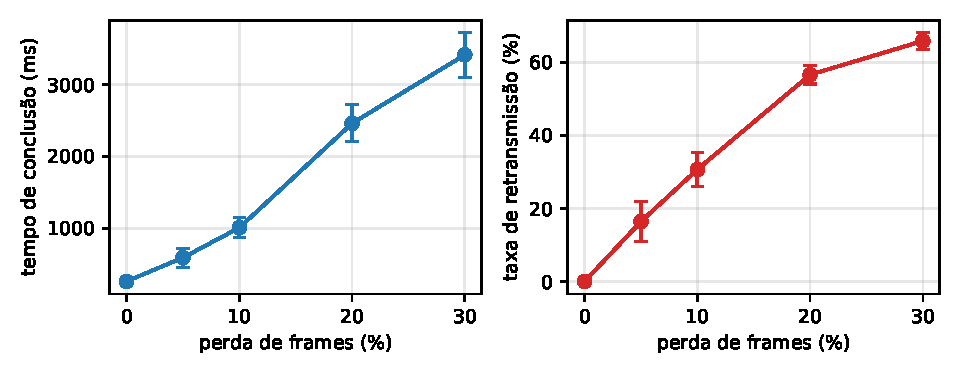
\includegraphics[width=0.92\textwidth]{fig_loss.pdf}
\caption{Tempo de conclus\~ao e taxa de retransmiss\~ao em fun\c{c}\~ao da perda (barras: desvio padr\~ao).}
\label{fig:loss}
\end{figure}

\subsection{Impacto do atraso na rede}

\begin{table}[H]
\centering\small
\begin{adjustbox}{max width=\textwidth}\begin{tabular}{rrrrrr}
\toprule
Atraso por salto (ms) & Tempo, janela 1 (ms) & Tempo, janela 4 (ms) & Tempo, janela 16 (ms) & RTT medido (ms) & $2\times$ atraso (ms) \\
\midrule
0 & 1 & 1 & 1 & 0,0 & 0 \\
5 & 520 & 135 & 42 & 10,4 & 10 \\
10 & 1023 & 273 & 82 & 20,5 & 20 \\
20 & 2027 & 526 & 163 & 40,5 & 40 \\
50 & 5023 & 1306 & 402 & 100,5 & 100 \\
\bottomrule
\end{tabular}
\end{adjustbox}
\caption{Tempo de conclus\~ao de 50 mensagens, por atraso e tamanho de janela.}
\end{table}

O tempo de conclus\~ao segue de perto o modelo $\lceil N/w \rceil \times \text{RTT}$. Com 50~ms de atraso por salto e RTT medido de 100,5~ms, a janela 1 leva 5023~ms (modelo: $50 \times 100{,}5 = 5025$~ms), a janela 4 leva 1306~ms (modelo: $13 \times 100{,}5 = 1306{,}5$~ms) e a janela 16 leva 402~ms (modelo: $4 \times 100{,}5 = 402$~ms). O RTT medido tamb\'em acompanha o dobro do atraso configurado (10,4~ms para 10~ms, 100,5~ms para 100~ms; o excedente vem do processamento). A janela maior compensa o atraso mantendo mais segmentos em voo, mas com perdas o ganho diminui (Tabela~\ref{tab:window}): com 20~ms de atraso, a janela 16 \'e 15,0 vezes mais r\'apida que a janela 1 sem perdas e apenas 3,7 vezes mais r\'apida com 10\% de perda.

\begin{figure}[H]
\centering
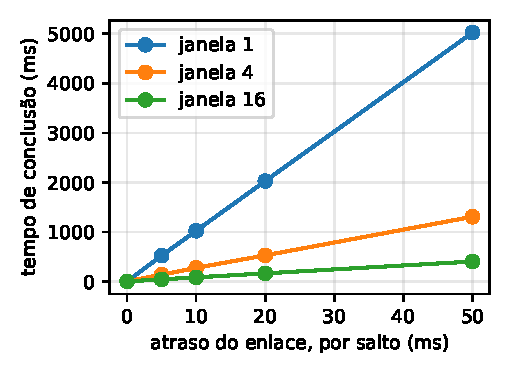
\includegraphics[width=0.55\textwidth]{fig_delay.pdf}
\caption{Tempo de conclus\~ao em fun\c{c}\~ao do atraso, para tr\^es tamanhos de janela.}
\end{figure}

\subsection{Taxa de retransmiss\~ao e tamanho da janela}

Os valores da Tabela~\ref{tab:loss} e da Figura~\ref{fig:loss} j\'a mostram a taxa de retransmiss\~ao em fun\c{c}\~ao da perda. A taxa tamb\'em reage \`a corrup\c{c}\~ao quando o CRC est\'a ativo, pois um frame rejeitado equivale a um frame perdido: com 20\% de corrup\c{c}\~ao, as retransmiss\~oes sobem de zero para 96 por 100 mensagens (Tabela~\ref{tab:corruption}). A Tabela~\ref{tab:window} separa o efeito da janela. Sem perdas, o ganho da janela segue o modelo ($4{,}0$ e $15{,}0$ vezes, como previsto para 60 mensagens). Com perdas, o ganho encolhe e a taxa de retransmiss\~ao cresce com a janela, porque o \emph{go-back-N} reenvia mais segmentos a cada expira\c{c}\~ao: a janela maior termina antes quando o atraso \'e grande, mas ao custo de bem mais tr\'afego redundante.

\begin{table}[H]
\centering\small
\begin{adjustbox}{max width=\textwidth}\begin{tabular}{rrrrrr}
\toprule
Perda & Atraso (ms) & Janela & Tempo (ms) & Ganho sobre a janela 1 & Taxa de retransmiss\~ao (\%) \\
\midrule
0\% & 20 & 1 & 2434 $\pm$ 3 & 1,0 & 0,0 $\pm$ 0,0 \\
0\% & 20 & 4 & 608 $\pm$ 1 & 4,0 & 0,0 $\pm$ 0,0 \\
0\% & 20 & 16 & 163 $\pm$ 0 & 15,0 & 0,0 $\pm$ 0,0 \\
10\% & 20 & 1 & 4771 $\pm$ 293 & 1,0 & 21,7 $\pm$ 2,1 \\
10\% & 20 & 4 & 1767 $\pm$ 505 & 2,7 & 31,0 $\pm$ 9,5 \\
10\% & 20 & 16 & 1293 $\pm$ 363 & 3,7 & 60,7 $\pm$ 8,8 \\
30\% & 5 & 1 & 5037 $\pm$ 693 & 1,0 & 54,8 $\pm$ 3,9 \\
30\% & 5 & 4 & 2104 $\pm$ 298 & 2,4 & 66,9 $\pm$ 3,3 \\
30\% & 5 & 16 & 1486 $\pm$ 227 & 3,4 & 84,0 $\pm$ 2,0 \\
\bottomrule
\end{tabular}
\end{adjustbox}
\caption{Efeito do tamanho da janela com e sem perdas (60 mensagens, 3 execu\c{c}\~oes; atraso de 20~ms, e de 5~ms na linha de 30\% de perda).}
\label{tab:window}
\end{table}

A Figura~\ref{fig:window_sweep} mostra que esse ganho tem limite. Com 5\% de perda e atraso de 1~ms (300 mensagens), o tempo m\'edio cai de 3703~ms com janela 1 para 1372~ms com janela 8 e n\~ao melhora depois (de 1347 a 1524~ms nas janelas de 16 a 64, dentro da variabilidade), enquanto a taxa de retransmiss\~ao sobe de 11,1\% para 75,5\%. O contador de expira\c{c}\~oes do temporizador explica o patamar: o tempo m\'edio fica pr\'oximo de $\text{expira\c{c}\~oes} \times \text{RTO}$ (16,0 expira\c{c}\~oes $\times$ 80~ms $= 1280$~ms para a janela 16, contra 1347~ms medidos), e o n\'umero de expira\c{c}\~oes fica entre 15,7 e 19,0 a partir da janela 2. Cada perda de dado custa um temporizador inteiro, pois n\~ao h\'a retransmiss\~ao antecipada por ACKs duplicados, e uma janela maior n\~ao reduz o n\'umero de perdas. Com janela 1, as 37,7 expira\c{c}\~oes tamb\'em incluem ACKs perdidos, o que sugere que nas janelas maiores o ACK cumulativo seguinte mascara esse tipo de perda. Nessas condi\c{c}\~oes, uma janela moderada (4 a 8) basta, e janelas maiores s\'o aumentam o tr\'afego redundante.

\begin{figure}[H]
\centering
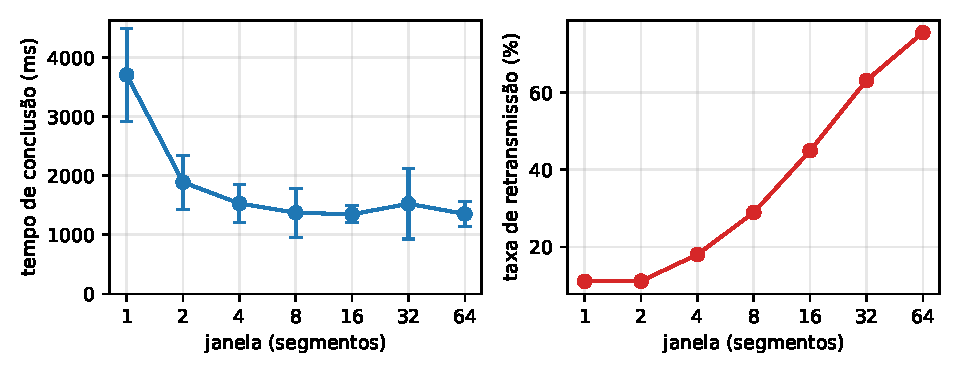
\includegraphics[width=0.92\textwidth]{fig_window_sweep.pdf}
\caption{Tempo de conclus\~ao e taxa de retransmiss\~ao em fun\c{c}\~ao da janela, com 5\% de perda e 1~ms de atraso (300 mensagens, 3 execu\c{c}\~oes).}
\label{fig:window_sweep}
\end{figure}

Com atraso e sem perda a taxa \'e zero, desde que o temporizador seja maior que o RTT; por isso, no experimento de atraso, o temporizador acompanha o atraso ($4d + 60$~ms).

\subsection{Overhead introduzido pelas camadas}

\begin{table}[H]
\centering\small
\begin{adjustbox}{max width=\textwidth}\begin{tabular}{rrrrr}
\toprule
Mensagem (B) & Confi\'avel, medido & Confi\'avel, previsto & N\~ao confi\'avel, medido & N\~ao confi\'avel, previsto \\
\midrule
5 & 11,4 & 11,4 & 6,2 & 6,2 \\
10 & 6,2 & 6,2 & 3,6 & 3,6 \\
50 & 2,04 & 2,04 & 1,52 & 1,52 \\
100 & 1,52 & 1,52 & 1,26 & 1,26 \\
250 & 1,208 & 1,208 & 1,104 & 1,104 \\
500 & 1,104 & 1,104 & 1,052 & 1,052 \\
1000 & 1,052 & 1,052 & 1,026 & 1,026 \\
\bottomrule
\end{tabular}
\end{adjustbox}
\caption{Overhead: bytes no enlace por byte entregue pela aplica\c{c}\~ao.}
\end{table}

Cada frame de dados carrega 26 bytes de cabe\c{c}alhos (13 do transporte, 9 da rede e 4 do enlace), e cada ACK \'e um frame de 26 bytes sem carga \'util. O modo confi\'avel paga, portanto, $52$ bytes por mensagem, e o n\~ao confi\'avel, $26$: o overhead \'e $(S + 52)/S$ e $(S + 26)/S$ para mensagens de $S$ bytes. Os valores medidos coincidem exatamente com essas f\'ormulas. O custo \'e alto para mensagens pequenas (11,4 vezes para 5 bytes, no modo confi\'avel) e tende a 1 para mensagens grandes (1,052 para 1000 bytes). O transporte responde por metade dos 26 bytes, a rede por 35\% e o enlace por 15\%. Os cabe\c{c}alhos IP e UDP reais, que ficam abaixo do meio simulado (28 bytes por datagrama), n\~ao entram na conta.

\begin{figure}[H]
\centering
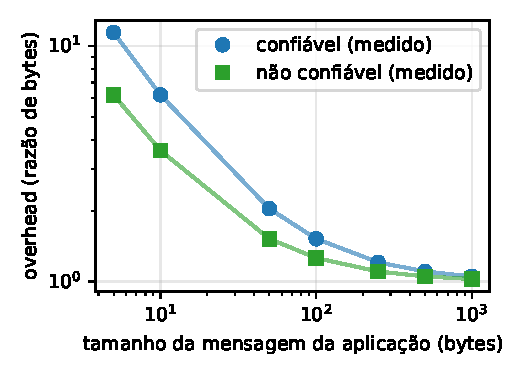
\includegraphics[width=0.55\textwidth]{fig_overhead.pdf}
\caption{Overhead medido (pontos) e previsto (linhas) em fun\c{c}\~ao do tamanho da mensagem.}
\end{figure}

\subsection{Comunica\c{c}\~ao confi\'avel e n\~ao confi\'avel}

\begin{table}[H]
\centering\small
\begin{adjustbox}{max width=\textwidth}\begin{tabular}{llrrrr}
\toprule
Perda & Transporte & Entregues (\%) & Tempo (ms) & Bytes no enlace (KiB) & Retransmiss\~oes \\
\midrule
0\% & confi\'avel & 100,0 $\pm$ 0,0 & 260 $\pm$ 1 & 14,8 $\pm$ 0,0 & 0 $\pm$ 0 \\
0\% & n\~ao confi\'avel & 100,0 $\pm$ 0,0 & n.a. & 12,3 $\pm$ 0,0 & 0 $\pm$ 0 \\
10\% & confi\'avel & 100,0 $\pm$ 0,0 & 1006 $\pm$ 139 & 21,1 $\pm$ 1,4 & 45 $\pm$ 9 \\
10\% & n\~ao confi\'avel & 89,7 $\pm$ 3,2 & n.a. & 12,3 $\pm$ 0,0 & 0 $\pm$ 0 \\
20\% & confi\'avel & 100,0 $\pm$ 0,0 & 2463 $\pm$ 255 & 32,9 $\pm$ 1,8 & 131 $\pm$ 14 \\
20\% & n\~ao confi\'avel & 75,3 $\pm$ 5,7 & n.a. & 12,3 $\pm$ 0,0 & 0 $\pm$ 0 \\
30\% & confi\'avel & 100,0 $\pm$ 0,0 & 3430 $\pm$ 328 & 41,3 $\pm$ 2,5 & 194 $\pm$ 19 \\
30\% & n\~ao confi\'avel & 67,7 $\pm$ 6,0 & n.a. & 12,3 $\pm$ 0,0 & 0 $\pm$ 0 \\
\bottomrule
\end{tabular}
\end{adjustbox}
\caption{Transporte confi\'avel e n\~ao confi\'avel sob perda (100 mensagens, 3 execu\c{c}\~oes).}
\end{table}

O modo n\~ao confi\'avel entrega aproximadamente a fra\c{c}\~ao $1 - p$ das mensagens (89,7\%, 75,3\% e 67,7\% para $p$ igual a 10, 20 e 30\%, contra os 90, 80 e 70\% esperados; a diferen\c{c}a est\'a dentro da variabilidade de tr\^es execu\c{c}\~oes de 100 mensagens), e o receptor detecta as lacunas pela numera\c{c}\~ao. O modo confi\'avel entrega 100\% em todos os casos, ao custo de mais bytes no enlace (14,8~KiB sem perdas, contra 12,3~KiB, por causa dos ACKs; 41,3~KiB com 30\% de perda) e de tempo. O tempo do modo n\~ao confi\'avel n\~ao \'e compar\'avel, pois o emissor termina assim que envia, sem esperar confirma\c{c}\~ao. Os tempos do modo confi\'avel repetem a configura\c{c}\~ao da Se\c{c}\~ao~7.1 em execu\c{c}\~oes independentes e por isso diferem em menos de 1\% dos de l\'a (por exemplo, 3430~ms contra 3413~ms com 30\% de perda).

\begin{figure}[H]
\centering
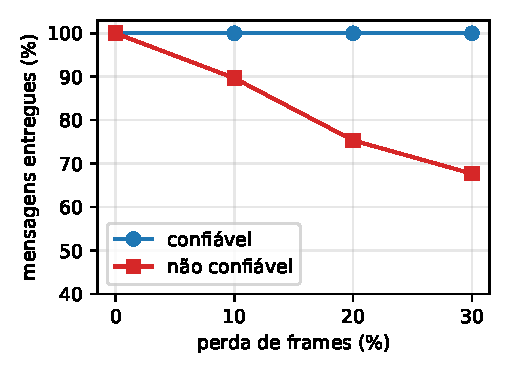
\includegraphics[width=0.55\textwidth]{fig_reliability.pdf}
\caption{Mensagens entregues em fun\c{c}\~ao da perda, nos dois modos.}
\end{figure}

\subsection{Detec\c{c}\~ao de erros no enlace}

\begin{table}[H]
\centering\small
\begin{adjustbox}{max width=\textwidth}\begin{tabular}{llrrrr}
\toprule
Corrup\c{c}\~ao & Enlace & \'Integras (\%) & Adulteradas na app & Frames rejeitados (CRC) & Retransmiss\~oes \\
\midrule
0\% & com CRC & 100,0 $\pm$ 0,0 & 0,0 $\pm$ 0,0 & 0,0 $\pm$ 0,0 & 0,0 $\pm$ 0,0 \\
0\% & sem CRC & 100,0 $\pm$ 0,0 & 0,0 $\pm$ 0,0 & 0,0 $\pm$ 0,0 & 0,0 $\pm$ 0,0 \\
5\% & com CRC & 100,0 $\pm$ 0,0 & 0,0 $\pm$ 0,0 & 12,0 $\pm$ 6,1 & 24,0 $\pm$ 12,0 \\
5\% & sem CRC & 94,3 $\pm$ 3,1 & 5,7 $\pm$ 3,1 & 0,0 $\pm$ 0,0 & 6,7 $\pm$ 4,6 \\
10\% & com CRC & 100,0 $\pm$ 0,0 & 0,0 $\pm$ 0,0 & 26,0 $\pm$ 8,2 & 47,7 $\pm$ 17,0 \\
10\% & sem CRC & 91,3 $\pm$ 2,3 & 8,7 $\pm$ 2,3 & 0,0 $\pm$ 0,0 & 5,3 $\pm$ 4,6 \\
20\% & com CRC & 100,0 $\pm$ 0,0 & 0,0 $\pm$ 0,0 & 66,3 $\pm$ 15,6 & 96,0 $\pm$ 26,2 \\
20\% & sem CRC & 84,0 $\pm$ 5,3 & 16,0 $\pm$ 5,3 & 0,0 $\pm$ 0,0 & 19,0 $\pm$ 6,6 \\
\bottomrule
\end{tabular}
\end{adjustbox}
\caption{Corrup\c{c}\~ao de bits nos frames, com e sem verifica\c{c}\~ao do CRC-16.}
\label{tab:corruption}
\end{table}

Com o CRC ativo, nenhuma mensagem adulterada chega \`a aplica\c{c}\~ao em nenhum n\'ivel de corrup\c{c}\~ao: os frames inv\'alidos s\~ao rejeitados (66 por execu\c{c}\~ao com 20\% de corrup\c{c}\~ao) e o transporte os recupera por retransmiss\~ao, de modo que as 100 mensagens chegam \'integras. Sem o CRC, 5,7\%, 8,7\% e 16,0\% das mensagens chegam adulteradas com 5, 10 e 20\% de corrup\c{c}\~ao. O ponto central \'e que o transporte confi\'avel n\~ao ajuda nesse caso: o segmento corrompido \'e aceito, entregue e confirmado, ent\~ao n\~ao h\'a o que retransmitir. A confiabilidade fim a fim depende de a camada inferior detectar o erro.

\begin{figure}[H]
\centering
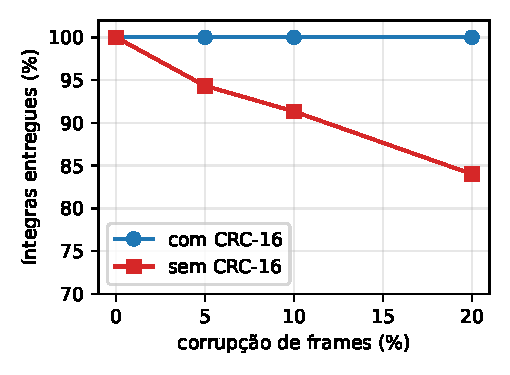
\includegraphics[width=0.55\textwidth]{fig_corruption.pdf}
\caption{Mensagens \'integras entregues, com e sem CRC-16.}
\end{figure}

\subsection{Valida\c{c}\~ao funcional}

Os testes automatizados (\texttt{make test}) somam 98 verifica\c{c}\~oes: 13 de codec e robustez e 85 de integra\c{c}\~ao entre processos.

Os de codec conferem o CRC contra o vetor padr\~ao (0x29B1 para ``123456789''), a ida e volta dos tr\^es cabe\c{c}alhos, a detec\c{c}\~ao de qualquer invers\~ao de um bit em um frame cujo pacote tem 100 bytes e a robustez diante de 200 mil entradas aleat\'orias nas quatro camadas.

Os de integra\c{c}\~ao cobrem a entrega confi\'avel sem perdas e com 25\% de perda, o modo n\~ao confi\'avel, a corrup\c{c}\~ao com e sem CRC, o encaminhamento em tr\^es n\'os, a expira\c{c}\~ao do TTL, a multiplexa\c{c}\~ao do chat e do benchmark no mesmo n\'o, a regra de separa\c{c}\~ao das camadas, a valida\c{c}\~ao dos argumentos e dos c\'odigos de sa\'ida (inclusive a desist\^encia quando o destino n\~ao existe), o intervalo entre mensagens, a rejei\c{c}\~ao de texto de chat fora de uma sess\~ao, a rejei\c{c}\~ao de mensagem de benchmark com identificador adulterado, o descarte de frames de origem desconhecida, a fila de atraso limitada a 2048 frames, o n\'umero exato de retransmiss\~oes antes de desistir, o efeito do jitter, as estat\'isticas exatas do receptor (lacunas e mensagens puladas), a demonstra\c{c}\~ao autom\'atica do encapsulamento (o trace da Se\c{c}\~ao~4) e as rela\c{c}\~oes medidas neste relat\'orio: a f\'ormula do overhead, o modelo $\lceil N/w \rceil \times \text{RTT}$ (inclusive para janelas acima de 64) e o efeito da janela sob perda.

O \emph{script} \texttt{fuzz\_protocol.py} (\texttt{make fuzz}) injeta, de forma determin\'istica, frames com CRC v\'alido e conte\'udo aleat\'orio ou mutado em todas as camadas, em tr\^es pap\'eis do n\'o (receptor com encaminhamento, iniciador de chat e emissor de benchmark), sob AddressSanitizer e UBSan.

O \texttt{conformance.py} confere, com um par escrito em Python que segue apenas o formato documentado, os campos dos tr\^es cabe\c{c}alhos, o CRC, o \emph{go-back-N}, o rein\'icio do temporizador, a sem\^antica do ACK cumulativo (inclusive duplicados e inv\'alidos), a amostragem de RTT sem retransmiss\~oes e o encaminhamento com TTL decrementado.

A su\'ite tamb\'em foi executada sob AddressSanitizer e UBSan (\texttt{make sanitize}), sem erros.

\section{Limita\c{c}\~oes e melhorias futuras}

\subsection{Limita\c{c}\~oes}
\begin{itemize}
  \item Sem fragmenta\c{c}\~ao: cada mensagem da aplica\c{c}\~ao cabe em um segmento de at\'e 1000 bytes.
  \item O \emph{go-back-N} reenvia a janela inteira, o que desperdi\c{c}a banda sob perda (Se\c{c}\~ao~7.3), e o receptor n\~ao guarda segmentos fora de ordem. Sem retransmiss\~ao antecipada por ACKs duplicados, cada perda de dado custa uma expira\c{c}\~ao inteira do temporizador, e janelas grandes aumentam o tr\'afego redundante sem reduzir o tempo.
  \item O temporizador de retransmiss\~ao \'e fixo e n\~ao h\'a controle de congestionamento, nem de fluxo al\'em do tamanho da janela.
  \item O CRC-16 detecta todos os erros de um bit e a maioria dos erros em rajada, mas n\~ao \'e infal\'ivel: erros aleat\'orios de v\'arios bits passam sem detec\c{c}\~ao com probabilidade da ordem de $2^{-16}$.
  \item Cada n\'o mant\'em no m\'aximo 16 fluxos de transporte, e os fluxos n\~ao expiram: um vizinho configurado pode esgotar a tabela variando as portas de origem, e os segmentos de novos fluxos passam a ser descartados.
  \item As rotas s\~ao est\'aticas, definidas na linha de comando; n\~ao h\'a descoberta de vizinhos nem roteamento din\^amico, e s\'o h\'a IPv4.
  \item As imperfei\c{c}\~oes s\~ao aplicadas por n\'o ao que ele envia; n\~ao h\'a reordena\c{c}\~ao dirigida de pacotes (a reordena\c{c}\~ao s\'o ocorre como efeito do jitter).
  \item Os experimentos rodam em \emph{loopback} com um n\'ucleo de CPU; os tempos absolutos dependem da m\'aquina, embora as tend\^encias e as rela\c{c}\~oes (como $\lceil N/w\rceil \times \text{RTT}$) n\~ao dependam.
\end{itemize}

\subsection{Melhorias futuras}
\begin{itemize}
  \item Retransmiss\~ao seletiva com buffer de recep\c{c}\~ao, para retransmitir apenas o que se perdeu, e retransmiss\~ao antecipada ap\'os ACKs duplicados.
  \item Estimativa adaptativa do RTT para o temporizador, com \emph{backoff} exponencial.
  \item Fragmenta\c{c}\~ao e remontagem de mensagens maiores que o segmento.
  \item Controle simples de congestionamento (por exemplo, janela que cresce e encolhe conforme perdas).
  \item Roteamento din\^amico por vetor de dist\^ancias entre os n\'os.
  \item Suporte a IPv6 e interface gr\'afica para visualizar o encapsulamento.
\end{itemize}

\end{document}
